% Einleitung
Dieses Kapitel stellt die grundlegenden Konzepte über Stents und faltende neuronale Netze vor, die für ein Verständnis dieser Arbeit benötigt werden. Der erste Unterabschnitt beginnt mit einer Einführung zu Stents und deren Einsatzgebiete in der Medizin. Des Weiteren wird das Herstellungsverfahren und die Geometrie des Aufbaus eines Stents erläutert. 

\mypar Das Kapitel beginnt mit einen kurzen Einblick in einige Verfahren des Histogrammausgleichs aus der Bildverarbeitung und wird mit den Grundlagen zu faltenden neuronalen Netzen fortgeführt. Hierbei wird sowohl in die Bausteine, als auch in die daraus bestehenden Netzwerkarchitekturen eingegangen. Zudem wird der Vorgang des Trainings eines neuronalen Netzes konkretisiert. 


% 2.1 Stents
\section{Stents}\label{sec:?}
Am 12. Juni 1986 veränderten Ulrich Sigwart und Jacques Puel, mit der ersten Anwendung eines Stents bei Menschen, die Behandlung der ischämischen Herzkrankheit. Es handelte sich um ein selbstexpandierendes geflochtenes Gittergewebe aus 16 Drähten mit einen Durchmesser von 60 $\mu$m. Wie in Abbildung \ref{fig:stent_view} zu sehen ist, war der Stent an einen Abgabekatheter durch eine einziehbare Plastikmembran gebunden. \cite{sigwart}

\begin{figure}[h!]
\centering
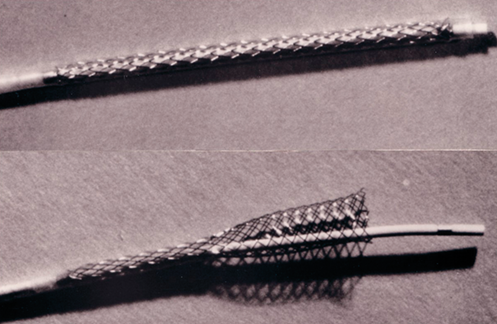
\includegraphics[width=9cm]{98_images/first_stent.png}
\caption{Der erste selbstexpandierbare Stent. Oben am Abgabekatheter gebunden. Unten zum Teil bereitgestellt durch Zurückziehen der Membran \cite{sigwart}.}
\label{fig:stent_view}
\end{figure}

\mypar Diese Art von Prothesen dienen als Instrument zum Offenhalten von Gefäßen oder Hohlorganen. Meistens bestehen diese aus Kunststoffen oder Metallen. Stents stabilisieren verengte Gefäße durch das Erweitern dieser und vermeiden einen erneuten Verschluss oder eine Verengung. Die Oberfläche des Gefäßes wird geglättet und Ablagerungen werden vom Stent gegen die Innenwand gepresst. Dies führt zu einer Verbesserung des Blutflusses im betroffenen Bereich. \cite{stent_def}


% Anwendungsgebiete
\subsection{Anwendungsgebiete}
Die Anwendung von Stents befindet sich bei der Aufdehnung verschlossener Gefäße oder Hohlorgane. Meist werden sie in den Koronararterien eingebaut, um diese zu stabilisieren. Auch Halsschlagadern, hirnversorgende Arterien, die Hauptschlagader sowie andere periphere Blutgefäße gehören zu den Einsatzgebieten von Stents. \cite{stent_def}

\mypar Zudem wird diese Kategorie von Prothesen auch in weiteren Bereichen eingesetzt. In der Speiseröhre und im Dickdarm werden Stents bei fortgeschrittenem Krebs verwendet. Ebenso finden sie im Harnleiter, in der Prostata, im Gallengang und seit wenigen Jahren auch in den Augen diverse Anwendung. 


% Herstellungsverfahren
\subsection{Herstellungsverfahren}
Eine schnelle Methode zur Produktion von Stents ist das Schneiden mit Lasern. Die thermische Energie des Lasers wird absorbiert, wodurch das Werkstück an definierten Stellen aufgewärmt und die zu entfernenden Stellen in einen geschmolzenen, verdampfenen oder chemisch veränderten Status transformiert werden. Anhand der Strömung eines Hochdruckgases können diese Anteile entfernt werden \cite{laser_cutting}. Da diese Methode für Strukturen eines kleineren Durchmessers ungeeignet ist, werden im Rahmen dieser Arbeit ausschließlich Stents untersucht, die durch einen Flechtprozess gefertigt werden. Eine Maschine zum Flechten von Stents ist in Abbildung \ref{fig:aufbau_flechten} zu sehen.

\mypar Auf einer ringförmigen Struktur werden mehrere Klöppel montiert, die jeweils eine Spule mit Flechtmaterial tragen. Beim Flechtvorgang dreht sich diese Struktur, sodass die Drähte um die Mitte gewickelt werden. Zudem drehen sich nebeneinanderstehende Klöppel in entgegengesetzte Richtungen, um die Gitterstruktur der Stents zu erzielen. \cite{flechten}

\begin{figure}[h!]
\centering
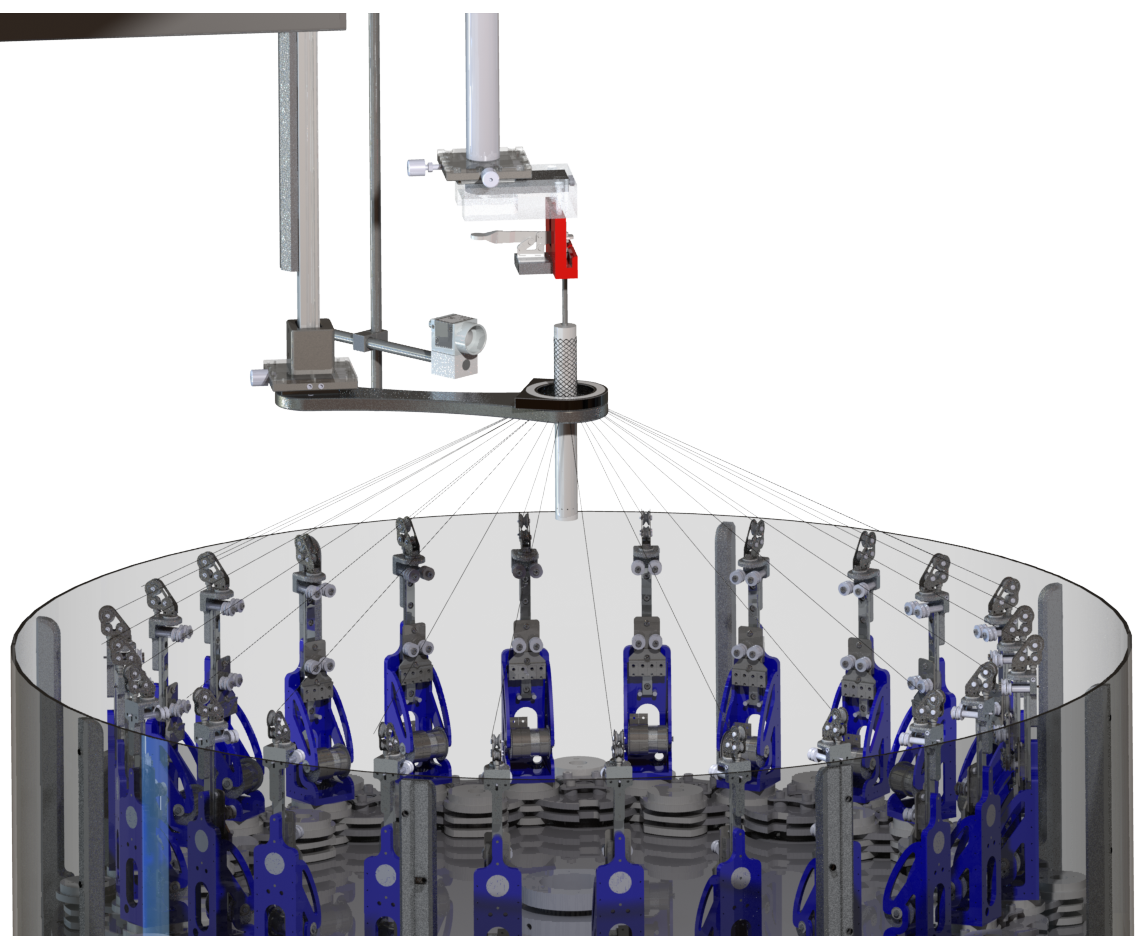
\includegraphics[width=7cm]{98_images/Flechtmaschine.png}
\caption{Aufbau einer Flechtmaschine, entnommen aus  \cite{flechtmaschine}}
\label{fig:aufbau_flechten}
\end{figure}


% Picklänge
\subsection{Picklänge}

Ein Stent kann als Gitter bestehend aus Rautenstrukturen aufgefasst werden. Eine solche Struktur, welche aus den Überkreuzungspunkten des Drahtes gebildet wird, wird als Pick bezeichnet. Die Picklänge entspricht in diesem Fall dem Abstand zwischen der oberen und unteren Ecke eines Picks. Diese Länge ist in Abbildung \ref{fig:picklaenge} dargestellt.

\begin{figure}[h!]
\centering
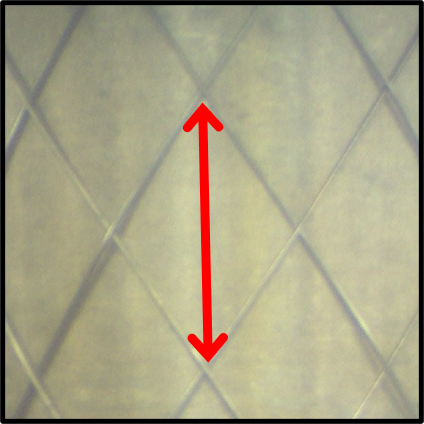
\includegraphics[width=5cm]{98_images/mittlerer_pick.png}
\caption{Veranschaulichung eines einzelnen Picks. Picklänge in rot visualisiert. Entnommen aus  \cite{flechtmaschine}.}
\label{fig:picklaenge}
\end{figure}


%
% 2.2 Histogrammausgleich
%
\section{Histogrammausgleich}\label{sec:histogramm-sec}
Der Histogrammausgleich ist ein Verfahren der Bildverarbeitung zur Kontrastverbesserung. Ziel ist es, ein Bild zu erhalten, bei dem die Bildwerte gleich verteilt sind \cite{automatische-sichtpruefung}. Ein Beispiel hierfür ist in Abbildung \ref{fig:ahe} dargestellt.

\begin{figure}[h!]
\centering
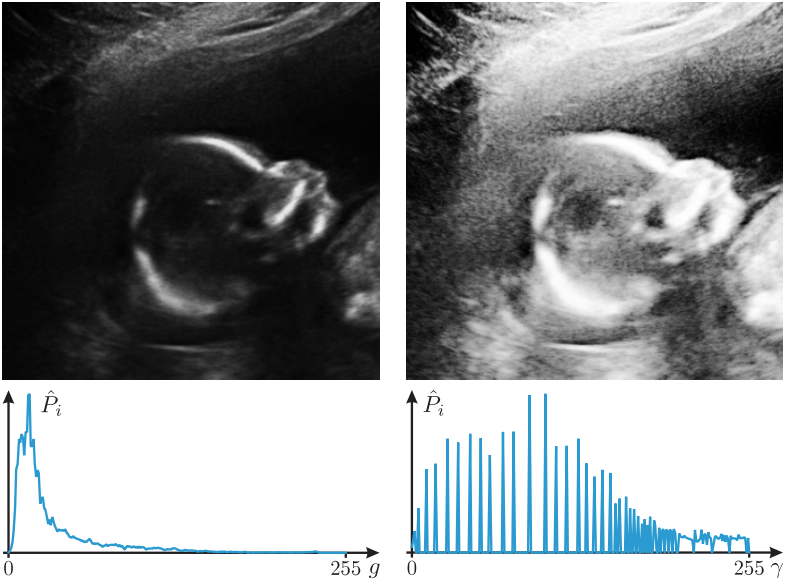
\includegraphics[width=11cm]{98_images/ahe.png}
\caption{Beispiel eines Histogrammausgleichs: links, ursprüngliches Bild; rechts, Ergebnis des Histogrammausgleichs. Darunter sind die zugehörigen Histogramme dargestellt. Entnommen aus \cite{automatische-sichtpruefung}.}
\label{fig:ahe}
\end{figure}


% AHE
\subsection{Adaptiver Histogrammausgleich}
Beim adaptiven Histogrammausgleich (engl. Adaptive Histogram Equalization) oder AHE wird diese Methode verbessert, sodass auch bei Bildern mit deutlich helleren oder dunkleren Regionen gute Ergebnisse erzielt werden können. Es werden mehrere Histogramme berechnet, um die Beleuchtungswerte im Bild neu zu verteilen. Jedes Pixel ändert sich basierend auf dem Histogramm der Region, von der es umgeben wird. Für die Anwendung an der am Rand liegenden Pixel wird ein sogenanntes Padding angewendet. In diesem Fall wird das Bild um die am Rand gespiegelten Werte erweitert. \cite{adaptive-hist-eq-and-its-variations}


% CLAHE
\subsection{Kontrastbegrenzter adaptiver Histogrammausgleich}\label{sec:clahe-sec}
Der kontrastbegrenzte adaptive Histogrammausgleich (engl. Contrast-Limited Adaptive Histogram Equalization (CLAHE)) ist eine Modifikation vom AHE. Abbildung \ref{fig:clahe} zeigt ein Beispiel für diese Methode. Hierbei wird die Kontrastverstärkung als die Ableitung der Transformationsfunktion, die Ein- und Ausgangsintensität verbindet, definiert. Der Ableitungswert eins entspricht keiner Verstärkung und höhere Werte führen zu höheren Verstärkungen. Um die Verstärkung zu begrenzen, wird das Histogramm an einer vordefinierten Höhe beschnitten. Somit wird die Steigung der Transformationsfunktion limitiert. Der Punkt, ab dem das Histogramm beschnitten wird, wird durch den Grenzwert der Steigung für die Funktion bestimmt. \cite{adaptive-hist-eq-and-its-variations}

\begin{figure}[h!]
\centering
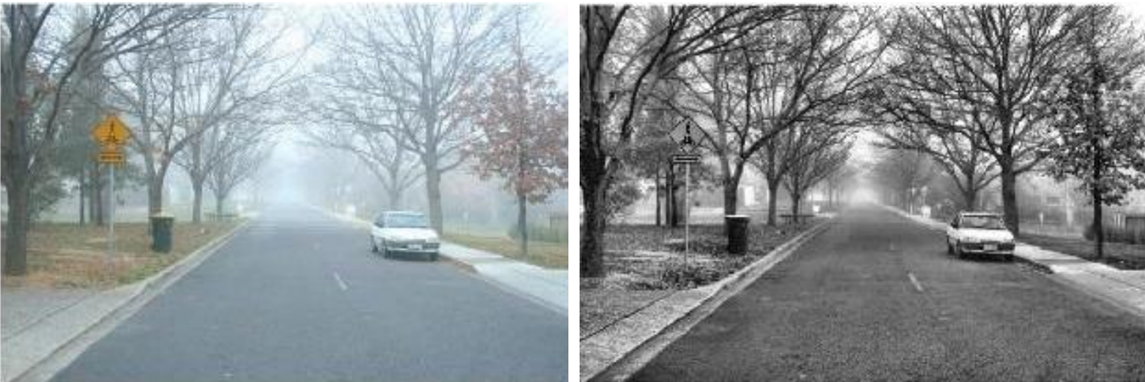
\includegraphics[width=10cm]{98_images/clahe.png}
\caption{Beispiel für die Anwendung von CLAHE: links, Originalbild mit Nebel; rechts, Bild nach der Anwendung von CLAHE. Entnommen aus \cite{clahe-based-enhancement-for-video}.}
\label{fig:clahe}
\end{figure} 


%
% 2.3 Deep Learninng
%
\section{Deep Learning}\label{sec:?}
Laut dem Wörterbuch der University of Cambridge ist Deep Learning eine Art künstlicher Intelligenz, die Algorithmen verwendet, welche auf der Funktionsweise des menschlichen Gehirns basieren \cite{cambridge_dl}. Diese neuronale Perspektive wird durch zwei Hauptideen vorangetrieben. Eine davon ist das Konzept der Nachkonstruktion der rechnerischen Prinzipien hinter dem Gehirn und die Duplizierung der Funktionalität dessen, um Intelligenz zu erschaffen. Zum anderen sollen Modelle des Deep Learnings nicht nur technischen Anwendungen dienen, sondern auch zu einem besseren Verstand über das Zerebrum und den Prinzipien, die der menschlichen Intelligenz zugrunde liegen, beitragen. \cite{Goodfellow-et-al-2016}

\begin{figure}[h!]
\centering
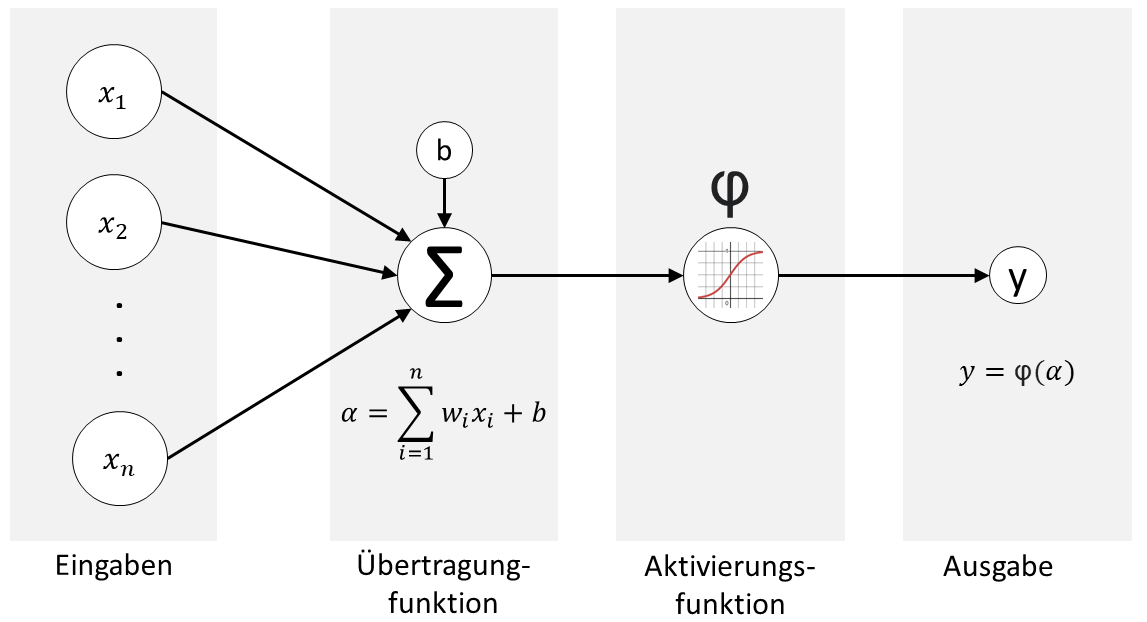
\includegraphics[width=12cm]{98_images/perceptron.png}
\caption{Schematischer Aufbau eines künstlichen neuronalen Netzes, das als einschichtiges Perzeptron-Netz modelliert wird. In Anlehnung an  \cite{Deep-Learning-mit-tf-keras-und-tfjs}.}
\label{fig:perceptron}
\end{figure}

\mypar Diese Modelle werden mithilfe künstlicher Neuronen gebildet, die auf mehreren Ebenen miteinander verbunden sind. Hierbei wird jede Nervenzelle als sogenanntes Perzeptron (siehe Abbildung \ref{fig:perceptron}) modelliert, bei dem die Dendriten des biologischen Neurons durch eine Schicht mit Eingaben gestaltet werden. Das Perikaryon wird durch die Übertragungsfunktion, das Axon durch die Ausgabe und die inhibitorischen bzw. exzitatorischen Eigenschaften der Synapse werden durch die Gewichte repräsentiert. Zur erwähnten Eingabe gehört auch ein Bias, welches zur Summe aller Eingaben addiert wird, bevor die Gleichung \ref{eq:uebertragungsfunktion_perzeptron} in die Aktivierungsfunktion eingegeben wird. Diese bestimmt den Schwellenwert, bei dem die Nervenzelle aktiviert wird \cite{Deep-Learning-mit-tf-keras-und-tfjs}. Somit war das von Frank Rosenblatt entworfene Perzeptron das erste Modell, welches in der Lage war, anhand von Beispielen die Gewichte der einzelnen Kategorien zu definieren \cite{The-Perceptron}.

\begin{equation}\label{eq:uebertragungsfunktion_perzeptron}
\alpha=\sum_{i=1}^{n}w_i x_i + b
\end{equation}

Mithilfe solcher künstlichen Neuronen kann ein neuronales Netz wie in Abbildung \ref{fig:mlp-fig} aufgebaut werden. Das abgebildete Netzwerk besteht aus drei Schichten: die Eingabeschicht, eine Zwischenschicht und eine Ausgabeschicht. Eine Eingabe wird in das Netz über die zwei Neuronen der ersten Schicht eingespeist und an die Zwischenschicht weitergeleitet. Von dort wird sie an die Ausgabeschicht geleitet, an der die Ausgabe des Netzwerks dargestellt wird.

\begin{figure}[h!]
\centering
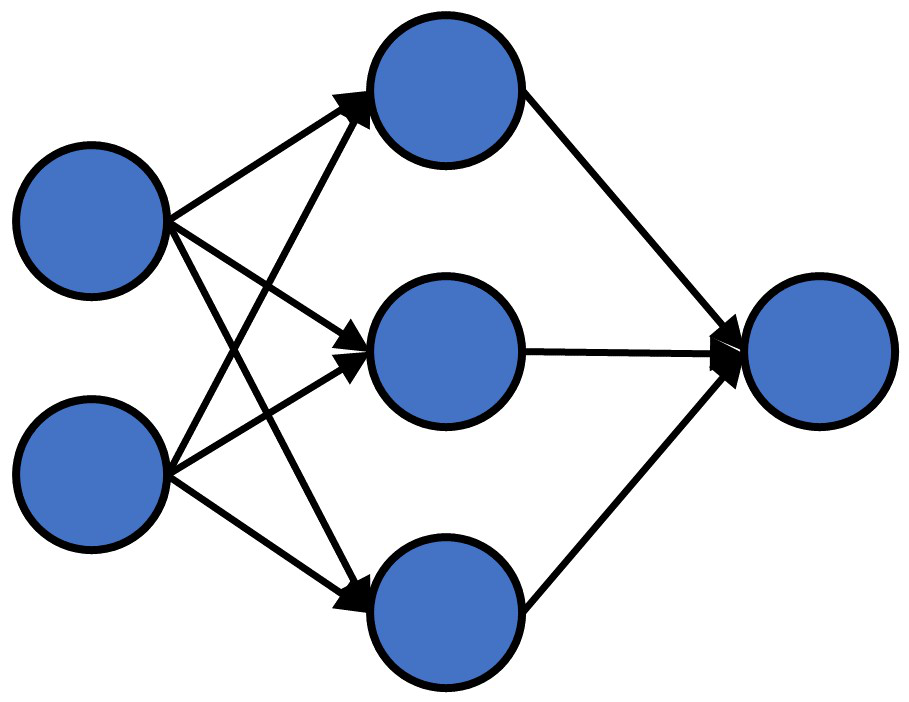
\includegraphics[width=6cm]{98_images/mlp.png}
\caption{Aufbau eines neuronalen Netzes mit zwei Neuronen für die Eingabe und einem für die Ausgabe}
\label{fig:mlp-fig}
\end{figure}


%
% Training eines Neuronalen Netzes
%
\subsection{Training eines neuronalen Netzes}
Das Training eines neuronalen Netzes ist der Prozess, bei dem die Parameter so gesetzt werden, dass die Differenz zwischen den Ist- und den Soll-Werten möglichst minimiert wird. Die Ausgabe des Netzes, also der Ist-Wert, wird mit der gewünschten Ausgabe (Soll-Wert), welche als Label bezeichnet wird, verglichen. \cite{cnns-an-overview-and-application-in-radiology}

\mypar Zu Beginn des Trainings wird ein Stapel (engl. batch) von Bildern wird vom Eingang zum Ausgang des Netzes vorwärts propagiert. Darauffolgend wird die Leistung des Modells mithilfe einer Fehlerfunktion berechnet. Diese misst die Differenz zwischen den Netzausgaben und den Labels. Im Anschluss werden die erlernbaren Parameter des Netzwerks anhand des Backpropagation-Algorithmus \cite{rumelhart1985learning} und dem Gradientenverfahren (siehe Abschnitt \ref{sec:gradient-descent-sec}) für Optimierungsprobleme angepasst. \cite{cnns-an-overview-and-application-in-radiology}

\mypar Der Ablauf des Trainings eines neuronalen Netzes wird in drei Phasen aufgeteilt, wodurch es drei unterschiedliche Datensätze benötigt: einen Test-, einen Validierungs- und einen Testdatensatz. Die Trainingsdaten werden verwendet, um das Modell zu trainieren. In der Validierungsphase wird bestimmt, wie gut das neuronale Netz trainiert wurde. Zuletzt wird der Testdatensatz für die Bewertung des Generalisierungsfehlers des Modells verwendet. \cite{hastie2009elements}


% MAE
\subsubsection{Mittlerer absoluter Fehler}\label{mae-section}
Der mittlere absolute Fehler (engl. Mean Absolute Error, kurz MAE) gibt den Durchschnitt aller Absolutbeträge der einzelnen Abweichungen zwischen der Netzausgabe und dem Label an. Für $n$ Testinstanzen wird dieser wie folgt berechnet:

\begin{equation}\label{eq:mae}
\text{MAE}=\frac{1}{n} \sum_{i=1}^{n} |(y_i - \lambda(x_i)|,
\end{equation}

\mypar wobei $y_i$ und $\lambda(x_i)$ den Soll- und Ist-Wert für $x_i$ darstellen. \cite{sammut2011encyclopedia}


% MSE
\subsubsection{Mittlerer quadratischer Fehler}
Beim mittleren quadratischen Fehler (engl. Mean Squared Error, kurz MSE) wird die quadratische Abweichung der Netzausgaben zum Soll-Wert über $n$ Testinstanzen wie folgt bestimmt: 

\begin{equation}\label{eq:mse}
\text{MSE}=\frac{1}{n} \sum_{i=1}^{n}(y_i-\lambda(x_i))^2.
\end{equation}

Die Bedeutungen für $y_i$, $\lambda(x_i)$ und $x_i$ sind analog zu \ref{mae-section}. \cite{sammut2011encyclopedia}

\mypar Der Unterschied zwischen den zwei vorgestellten Verlustfunktionen wird in Abbildung \ref{fig:mae-mse} anhand zwei beispielhafter Verläufe aufgezeigt. Der mittlere absolute Fehler steigt linear mit einem zunehmenden Fehler an. Im Gegensatz dazu steigt die Funktion beim MSE exponentiell mit einer Zunahme des Fehlers. Dadurch bestraft der mittlere quadratische Fehler große Abweichungen mehr als kleine.

\begin{figure}[h!]
\centering
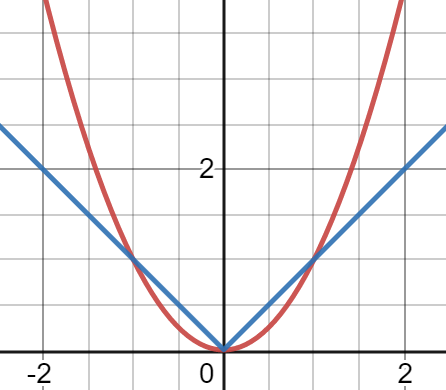
\includegraphics[width=5cm]{98_images/mae_mse.png}
\caption{Beispielhafter Verlauf für den mittleren absoluten Fehler (blau) und den mittleren quadratischen Fehler (rot).}
\label{fig:mae-mse}
\end{figure}


% Gradient Descent
\subsubsection{Gradientenverfahren}\label{sec:gradient-descent-sec}
Das Gradientenverfahren (engl. gradient descent) ist ein Optimierungsalgorithmus für das iterative Anpassen der erlernbaren Parameter eines neuronalen Netzes, um den Verlust des Netzwerks möglichst zu minimieren. Der Gradient der Verlustfunktion gibt die Richtung an, in der die negative Steigung der Funktion am größten ist. So werden die Filterkerne und Gewichte in diese Richtung des Gradienten angepasst. Die Schrittgröße wird anhand der Lernrate, ein positiver Skalar, bestimmt. Eine Darstellung dieses Verfahrens wird in Abbildung \ref{fig:grad-descent} dargestellt. Bei einer zu großen Lernrate kann die Verlustfunktion steigen anstatt zu sinken. Andernfalls wird das Training eines Netzes bei einer zu kleinen Lernrate langsamer und es besteht die Gefahr, bei einem hohen Fehler dauerhaft stecken zu bleiben \cite{Goodfellow-et-al-2016}. \cite{cnns-an-overview-and-application-in-radiology}

\begin{figure}[h!]
\centering
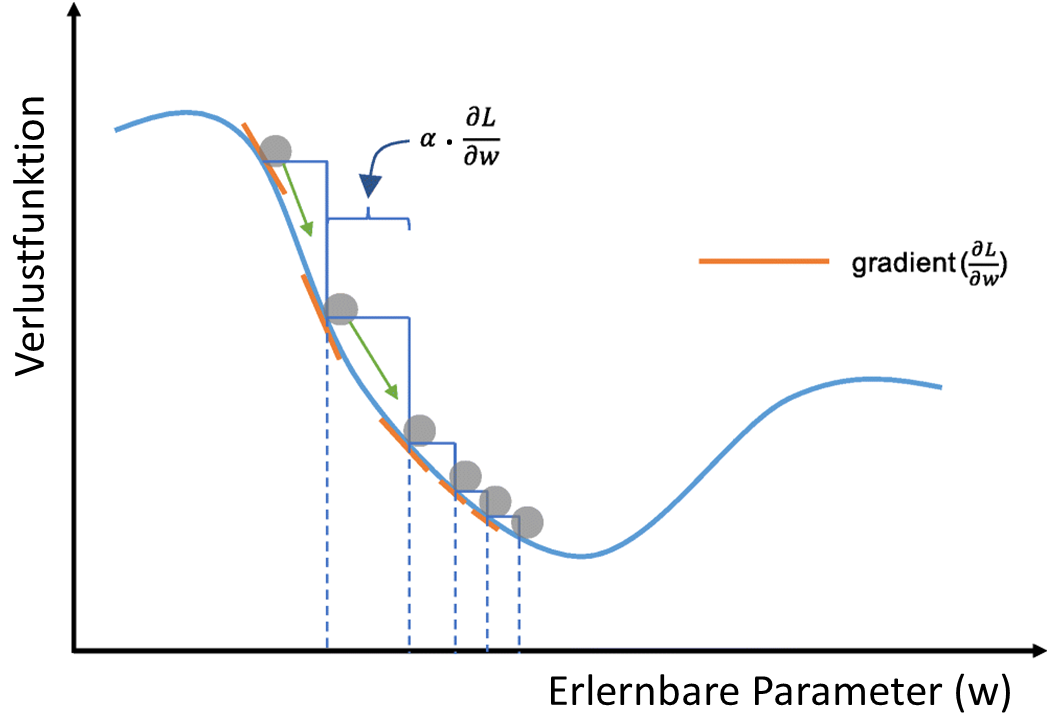
\includegraphics[width=10cm]{98_images/gradientenverfahren.png}
\caption{Verlauf des Gradientenverfahrens mit einer Lernrate $\alpha$, einer Verlustfunktion L und den Parametern w. Ursprüngliches Bild aus \cite{cnns-an-overview-and-application-in-radiology}.}
\label{fig:grad-descent}
\end{figure}

\mypar Eine solche Aktualisierung der Parameter wird in Gleichung \ref{eq:gradient-descent} formuliert. In diesem Fall steht $w$ für einen einzelnen Parameter, $\alpha$ für die Lernrate und $L$ für die Verlustfunktion.

\begin{equation}\label{eq:gradient-descent}
w:=w-\alpha \cdot \frac{\partial L}{\partial w}. 
\end{equation}


% Adam
\subsubsection{Adam}
Der Optimierungsalgorithmus Adam ist eine Weiterentwicklung des Gradientenverfahrens. Dieses Verfahren berechnet einzelne anpassungsfähige Lernraten für unterschiedliche Parameter und basiert auf zwei anderen Algorithmen und entnimmt deren Vorteile; AdaGrad und RMSProp. Adaptive Gradient (AdaGrad) stellt eine feste Lernrate pro Parameter fest und verbessert die Leistung bei sogenannten ''sparse''-Gradienten \cite{adagrad}. Laut Elibol et al. \cite{variance-red-w-sparse-grads} sind damit Gradienten gemeint, die eine geringe Anzahl an großen Koordinaten besitzen. Root Mean Square Propagation (RMSProp) verwendet den Durchschnitt des quadratischen Gradienten, um die Parameter anzupassen \cite{rmsprop}. Adam ist rechnerisch effizient, benötigt wenig Speicher und ist gut für Anwendungen mit vielen Daten und Parametern geeignet. \cite{adam-paper}

\mypar Die Parameteranpassungen werden wie folgt durchgeführt:

\begin{equation}\label{eq:adam1}
\theta_t = \theta_{t-1}-\alpha \frac{\hat{m}_t}{\sqrt{\hat{v}_t}+\epsilon}
\end{equation}

\mypar mit

\begin{equation}\label{eq:adam2}
\begin{aligned}
g_t = \nabla_{\theta} f_t(\theta_{t-1}) \\
m_t = \beta_1 m_{t-1} + (1-\beta_1)g_t \\
v_t = \beta_2 v_{t-1} + (1-\beta_2)g^2_t \\
\hat{m}_t = \frac{m_t}{1-\beta^t_1} \\
\hat{v}_t = \frac{v_t}{1-\beta^t_2}
\end{aligned}
\end{equation}

\mypar $\alpha$ steht für die Lernrate mit einem Wert von 1e-3 in der Veröffentlichung. $\epsilon$ ist eine sehr kleine Zahl, üblicherweise 1e-8 or 1e-10, um eine Nulldivision zu vermeiden. $\beta_1$ und $\beta_2$ sind die exponentiellen Abnahmeraten für die Momentenschätzwerte erster und zweiter Ordnung und betragen üblicherweise 0,9 bzw. 0,999. Nach der Berechnung des Gradienten $g_t$ zum Zeitpunkt $t$ werden die verzerrten Schätzwerte für das statische Moment $m_t$ und für das Trägheitsmoment $v_t$ aktualisiert. Darauffolgend wird die Verzerrung dieser Werte korrigiert und es ergeben sich $\hat{m}_t$ und $\hat{v}_t$. Aus diesen Anteilen kann der angepasste Parameter mit Gleichung \ref{eq:adam1} bestimmt werden. \cite{Goodfellow-et-al-2016}


% Regularisierung
\subsubsection{Regularisierung}\label{sec:regularisierung-sec}
Neuronale Netze werden nach dem Training auf Bilder oder Daten, die in dem Modell noch nie zuvor eingegeben wurden, getestet. Somit kann untersucht werden, wie gut ein Modell Informationen generalisieren kann. Ein Netzwerk mit einer guten Generalisierungsfähigkeit kann gute Ergebnisse auf diesen Testdaten erzielen. Das sogenannte Overfitting tritt auf, wenn ein Modell die Trainingsdaten zwar gut verarbeiten kann, aber nicht die Testdaten. In diesem Fall hat sich das neuronale Netz viel zu gut an die Trainingsdaten angepasst und kann noch nie gesehene Muster deshalb schlecht verarbeiten. Abbildung \ref{fig:alexnet-log-scale} zeigt den Verlauf eines solchen Trainings. Im Gegensatz dazu wird bei einer schlechten Leistung sowohl im Trainings-, als auch im Testdatensatz von Underfitting gesprochen. Um dieses fundamentale Problem des Deep Learnings zu bekämpfen, gibt es mehrere Methoden die angewendet werden können, wie Daten-Augmentation, Verwendung von mehr Trainingsdaten, Regularisierung, Batch Normalization (siehe \ref{batch-normalization-sec}) oder Reduzieren der Modellkomplexität \cite{overfitting-mechanism-and-avoidance-in-dnl}. Im Folgenden wird auf einige Techniken der Regularisierung tiefer eingegangen. \cite{cnns-an-overview-and-application-in-radiology}

\begin{figure}[h!]
\centering
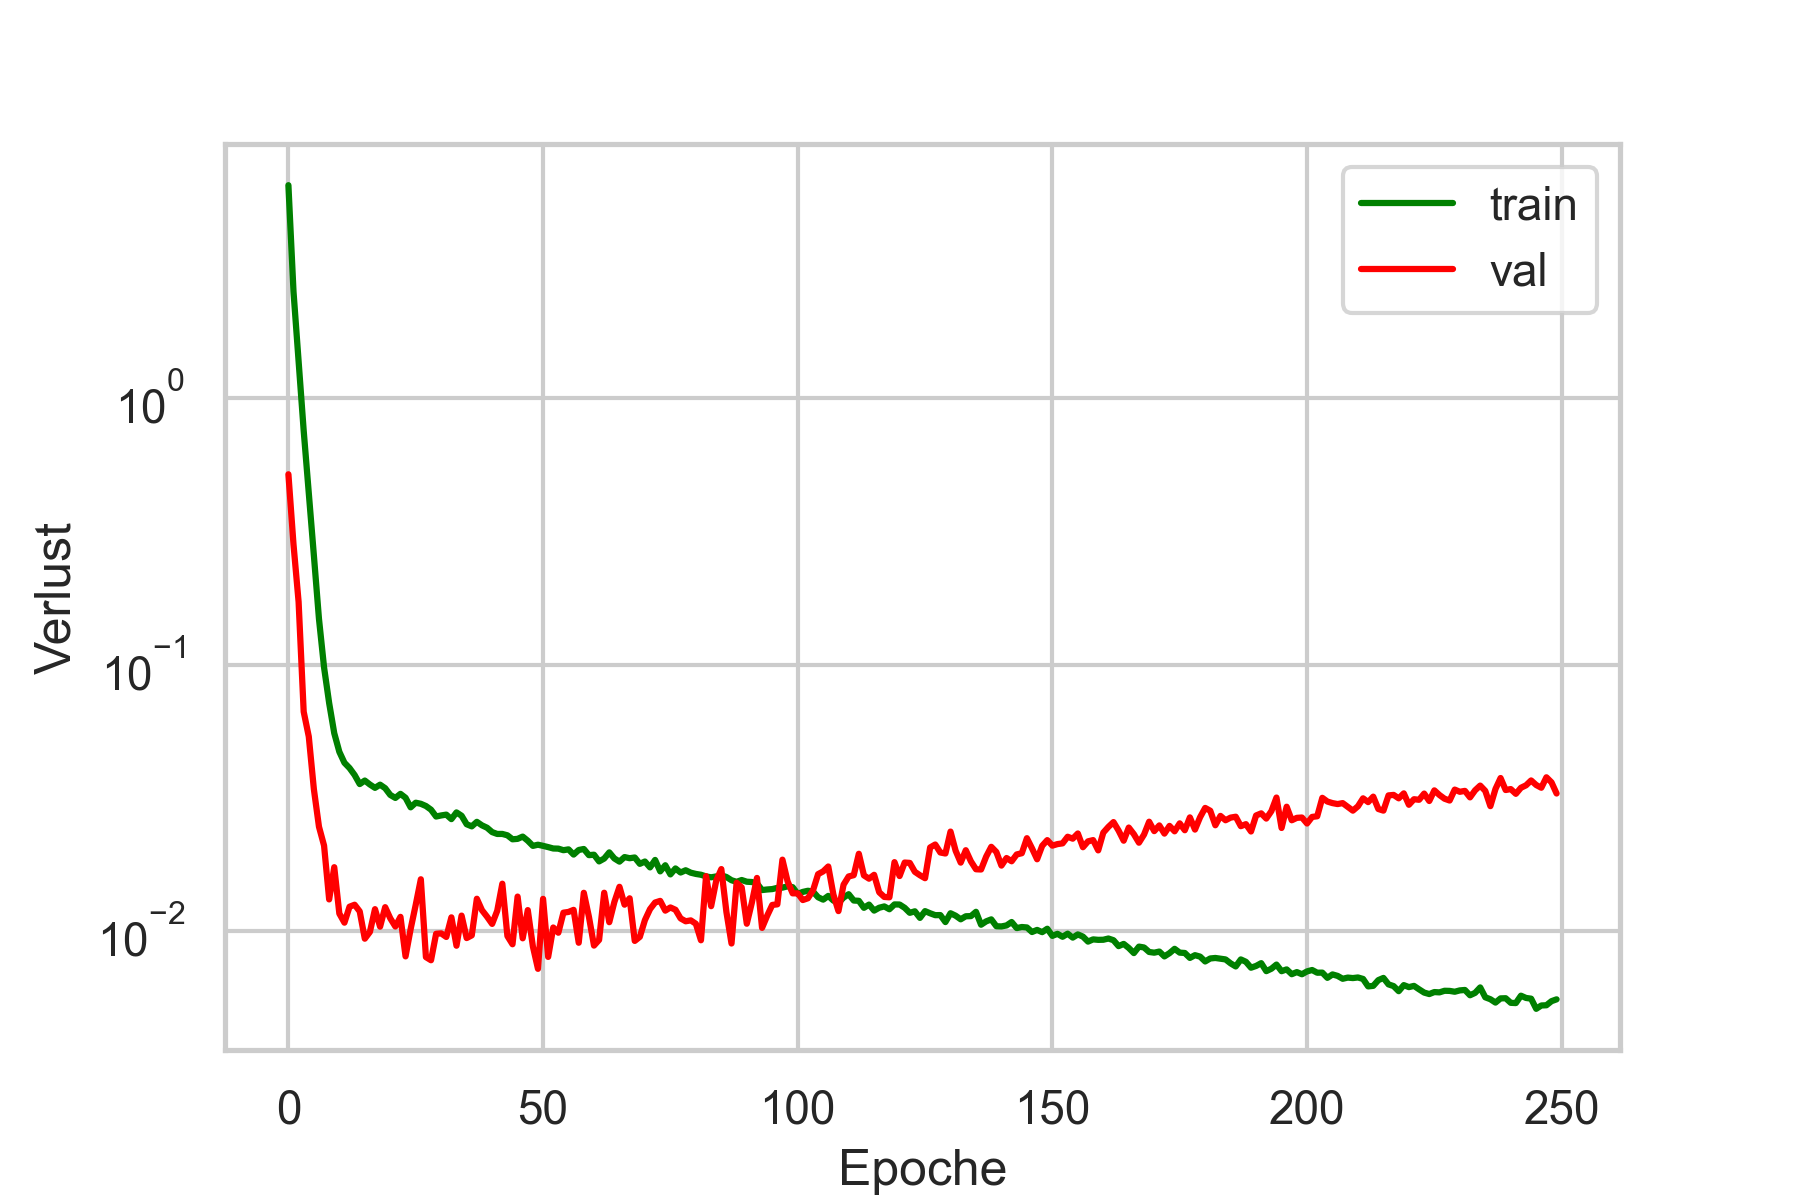
\includegraphics[width=12cm]{98_images/AlexNet_log_scale.png}
\caption{Beispielhafter Verlauf eines Trainings mit Overfitting. Der Trainingsloss sinkt über den gesamten Vorgang, demgegenüber fängt der Validierungsloss ab etwa der 50. Epoche an zu steigen.}
\label{fig:alexnet-log-scale}
\end{figure}

\mypar Eine verbreitete Methode ist das Early Stopping, welches für ein vorzeitiges Abbrechen des Trainingvorgangs, um Overfitting zu vermeiden, sorgt. Jedes Mal, wenn der Fehler auf dem Validierungssatz verringert wird, wird eine Kopie der Parameter gespeichert. Dieser Algorithmus beendet das Training, sobald das Modell nach einer vorgegebenen Anzahl an Iterationen keine besseren Ergebnisse auf die Validierungsdaten erzielt. Das Modell mit den besten Parametern wird zurückgegeben. \cite{Goodfellow-et-al-2016}

\mypar Das Dropout ist ein weiteres Instrument der Regularisierung. Beim Dropout wird während des Trainings ein Neuron und dessen Verbindungen mit einer vorgegebenen Ausfallwahrscheinlichkeit $p$ deaktiviert, wodurch das Neuron von der Modellarchitektur temporär ausgeschlossen wird. Während der Testphase sind alle Neuronen und Verbindungen aktiv, doch die Gewichte werden mit $p$ skaliert. Hiermit wird eine übermäße Abhängigkeit des Netzes von bestimmten Verbindungen vermieden. Dadurch wird anhand dieser Methode ein Ensemble trainiert, welches aus mehreren Teilnetzen besteht. Das Ensemble enthält alle möglichen Netzwerke, die durch Entfernen von Einheiten mit der Ausfallwahrscheinlichkeit gefertigt werden können. \cite{dropout}

\mypar Darüber hinaus sind die L1- und L2-Regularisierungen ein weiteres Mittel, um Overfitting zu vermeiden. Bei den Dabei handelt es sich um Funktionen, die zur Verlustfunktion hinzugefügt werden. Die L1-Regularisierung entspricht der Summe der Beträge, also die L1-Normen, der Parameter. Dies führt zu einer Lösung, bei der einige Parameter einen optimalen Wert von Null haben. Die Lösung ist also dünnbesetzter, wodurch sich das Netzwerk auf die Erkennung bedeutsamer Merkmale begrenzt. Bei der L2-Regularisierungsfunktion wird die L2-Norm der Parameter betrachtet. Dies verhindert das Entstehen von Gewichten mit zu hohen Werten. Formal sind die Bestrafungen der L1- und L2-Regularisierungen für eine Gewichtung $w_k$ in Gleichung \ref{eq:regularisierung-1} und Gleichung \ref{eq:regularisierung-2} definiert. \cite{deep-neural-network-regularization}

\begin{equation}\label{eq:regularisierung-1}
\Omega (W^{(p)})_{l1} = \vert w \vert  = \sum_{k=1}^{m} \vert w_k \vert
\end{equation}

\begin{equation}\label{eq:regularisierung-2}
\Omega(W^{(p)})_{l2} \equiv \Vert W \Vert^2_2
\end{equation}


% CNNs
\subsection{Faltende neuronale Netze}
Faltende neuronale Netze (kurz CNN) sind vorwärtsgekoppelte Netzwerkarchitekturen, weil sie durch unidirektionale Verbindungen zwischen den Neuronen ausgezeichnet werden. Dementsprechend führt kein Pfad aus dem Ausgang eines Neurons zum Eingang dessen oder zu einer vorherigen Schicht des Netzes; der Aufbau stellt einen azyklischen Graphen dar. Da sie von der von Hubel und Wiesel 1959 \cite{hubel-wiesel} erforschten Funktionsweise der Informationsverarbeitung im visuellen Kortex inspiriert sind, eignen sie sich besonders für Bilder. In dieser Region des Gehirns werden globale Probleme in mehrere kleinere und daher leichter zu lösende Schritte verwandelt. \cite{Deep-Learning-mit-tf-keras-und-tfjs}

\mypar Eine der ersten Implementierungen eines CNN ist das 1989 von LeCun et al. \cite{lenet-1} publizierte und neun Jahre später in \cite{lenet-2} verbesserte LeNet-5 Modell. Seitdem sind mehrere Architekturen und somit auch Schichten entworfen worden, mit dem Ziel, Schwierigkeiten beim Trainieren der Netze zu beseitigen und deren Effektivität zu steigern. \cite{recent-advances-in-cnns}


% Convolutional Layer
\subsubsection{Convolutional Layer}
Das Convolutional Layer (engl. Convolutional Neural Network, kurz Conv) ist ein grundlagender Bestandteil aller CNN-Architekturen, weil es für das Extrahieren von Eigenschaften sorgt. Dies basiert auf der mathematischen Operation der Faltung \cite{cnns-an-overview-and-application-in-radiology}. Die Faltung innerhalb der Schicht wird typischerweise wie in Gleichung \ref{eq:faltung} notiert.

\begin{equation}\label{eq:faltung}
S(i,j)=(I*K)(i,j)=\sum_{m}\sum_{n}I(m,n)K(i-m,j-n)
\end{equation}

\mypar Hierbei wird ein zweidimensionales Bild $I$ mit einem ebenfalls zweidimensionalen Filterkern gefalten und ergibt somit eine sogenannte Feature Map (siehe Abbildung \ref{fig:convolution}) \cite{Goodfellow-et-al-2016}. Der Filter wird auf die gesamte Eingabe angewendet. Durch die Wiederholung des Vorgangs mit unterschiedlichen Kernen kann eine willkürliche Anzahl an Feature Maps erzeugt werden, welche unterschiedliche Eigenschaften der Eingabe darstellen. So können unterschiedliche Feature Maps beispielsweise Augen, Mund und Nase auf Bildern von Gesichten hervorheben. Üblicherweise werden Filter der Größe $3 \times 3$ verwendet, doch diese lässt sich modifizieren. Der Abstand zwischen zwei Positionen an denen der Filterkern angewendet wird, wird durch dem Stride festgelegt. \cite{cnns-an-overview-and-application-in-radiology}

\begin{figure}[h!]
\centering
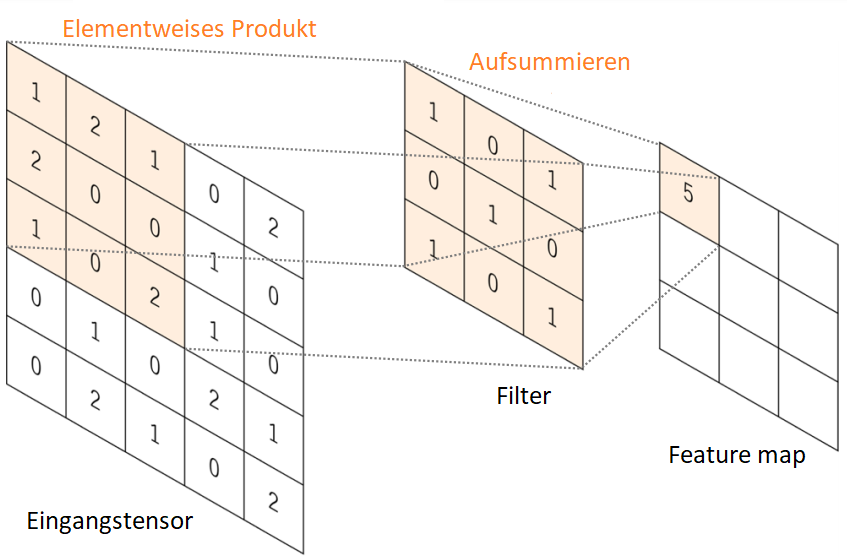
\includegraphics[width=11cm]{98_images/convolution.png}
\caption{Beispiel einer Faltungsoperation mit einen $3 \times 3$ Filter. Entnommen und neu beschriftet aus  \cite{cnns-an-overview-and-application-in-radiology}.}
\label{fig:convolution}
\end{figure}

\mypar Da die durch die Anwendung des Filters enstandene Feature Map eine reduzierte Höhe und Breite gegenüber dem ursprünglichem Bild aufweist, kann beispielsweise zero-Padding benutzt werden. An den Rändern der Eingabe werden Reihen und Spalten mit Nullen hinzugefügt, sodass die Dimension des Tensors, welches eine bestimmte Anzahl von Vektoren auf einen Vektor abbildet, beibehalten wird. \cite{an-introduction-to-cnns}


% Aktivierungsfunktionen
\subsubsection{Aktivierungsfunktionen}
Ausgaben einer linearen Operation wie die Faltung werden darauffolgend in eine nichtlineare Aktivierungsfunktion eingesetzt. Die Auswahl der Funktion hat einen signifikanten Einfluss auf das Training und die Leistung des Modells \cite{searching-for-act-functions}. Im Rahmen dieser Arbeit sind folgende drei Funktionen relevant. 

\mypar Die Sigmoid-Aktivierungsfunktion aus Gleichung \ref{eq:sigmoid} wird oftmals auch als logistische Funktion bezeichnet. Es handelt sich um eine begrenzt differenzierbare reelle Funktion, welche für reelle Eingabewerte definiert ist und Werte zwischen null und eins ausgibt. \cite{activation-functions}

\begin{equation}\label{eq:sigmoid}
f(x)=\frac{1}{1+e^{-x}}
\end{equation}

 Eine der bekanntesten Aktivierungsfunktionen ist die in Gleichung \ref{eq:relu} aufgezeigte Rectified Linear Unit (ReLU) \cite{imagenet-class-w-deep-cnns}. Künstliche neuronale Netze mit ReLU sind einfacher zu optimieren, als Netze, welche zuvor veröffentlichten Funktionen verwenden, weil die mathematischen Operationen der Funktion simpler sind \cite{searching-for-act-functions}.

\begin{equation}\label{eq:relu}
f(x)=\text{max}(0,x)
\end{equation}

\mypar Das Exponential Linear Unit (ELU) wurde 2015 eingeführt (siehe Gleichug \ref{eq:elu}) und erlaubt ein schnelleres und präziseres Lernen in Netzen. Im Vergleich zur ReLU-Funktion können ELUs auch negative Werte aufzeigen, beschleunigen das Training und verbessern die Generalisierung der Netze. \cite{elus}

\begin{equation}\label{eq:elu}
f(x)=
\begin{cases}
x & \text{, x} > \text{0} \\
\alpha(\text{exp}(x)-1) & \text{, x} \leqslant \text{0}
\end{cases}
\text{	für } \alpha > \text{0}
\end{equation}


% Pooling Layer
\subsubsection{Pooling Layer}
Ziel des Pooling Layers ist, die Dimensionalität der Eingabe zu reduzieren und gleichzeitig möglichst keinen Informationsverlust zu erleiden \cite{understanding-of-a-cnn}. Eine Invarianz gegen kleine Verschiebungen und Verzerrungen wird eingeführt und die Anzahl der erlernbaren Parameter sinkt. Ähnlich zur Faltung, sind Stride, Padding und die Größe des Filters Hyperparameter beim Pooling. Damit ist ein Parameter gemeint, dessen Wert zur Steuerung des Trainings verwendet wird. Eine der meist verbreiteten Formen ist das Max Pooling, welche in Abbildung \ref{fig:pooling-layer} angewendet wird, bei dem der höchste Wert innerhalb des Bereiches übergeben wird. Eine weitere Variante ist das Average Pooling, bei dem der durchschnittliche Wert aller Werte im Bereich übernommen wird. \cite {cnns-an-overview-and-application-in-radiology}

\begin{figure}[h!]
\centering
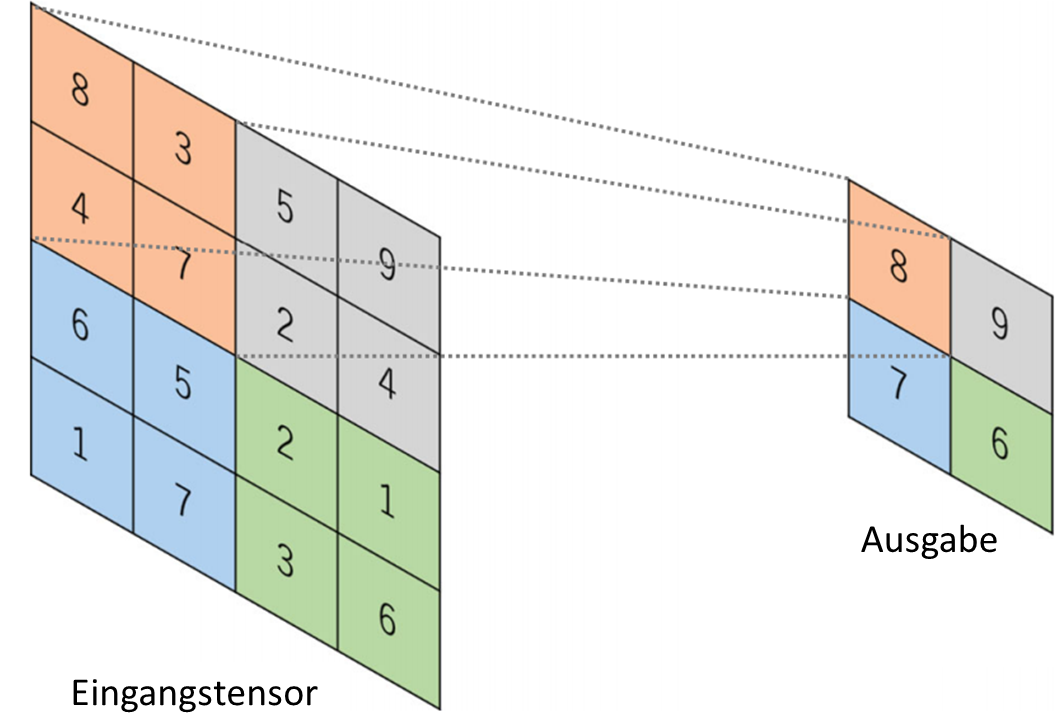
\includegraphics[width=10cm]{98_images/pooling_layer.png}
\caption{Beispiel zur Anwendung von Max Pooling. Ursprüngliches Bild aus \cite{cnns-an-overview-and-application-in-radiology}.}
\label{fig:pooling-layer}
\end{figure}


% Fully Connected Layer
\subsubsection{Fully Connected Layer}
Beim Fully Connected Layer (auch Dense Layer genannt) sind alle Neuronen direkt mit allen Neuronen der zwei benachbarten Schichten verbunden. Ein solcher Aufbau wird in Abbildung \ref{fig:fc-layer} aufgezeigt. Dies ist ähnlich zur Form in der die Nervenzellen beim einem traditionellen neuronalen Netz angeordnet sind. Da dieser Aufbau viele Paramter einbezieht, können sie eine lange Zeit beim Trainieren beanspruchen. \cite{understanding-of-a-cnn}

\begin{figure}[h!]
\centering
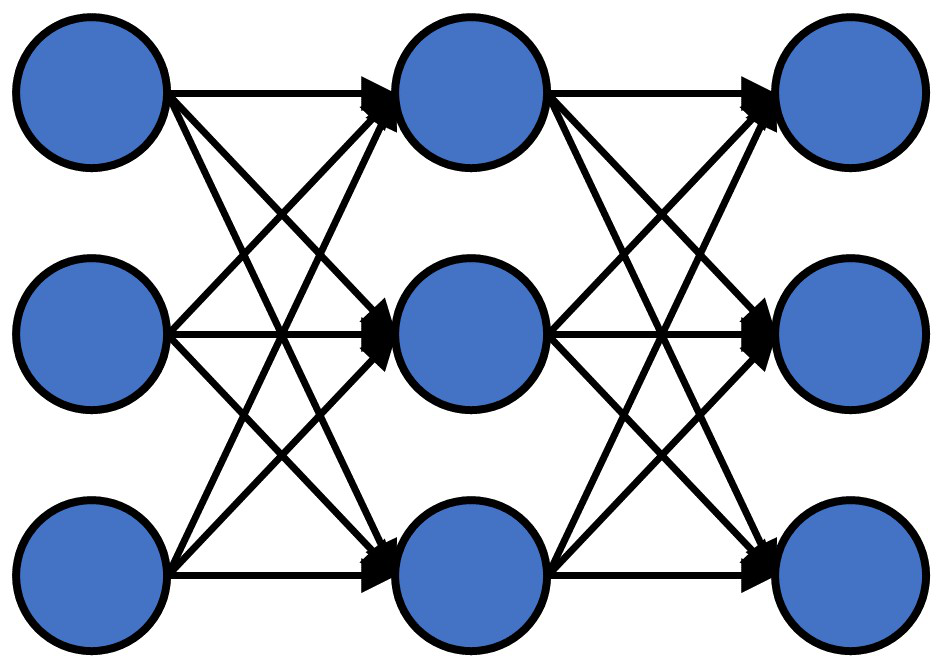
\includegraphics[width=5cm]{98_images/fc_layer.png}
\caption{Aufbau eines Fully Connected Layers.}
\label{fig:fc-layer}
\end{figure}


% Batch Normalization Layer
\subsubsection{Batch Normalization Layer}\label{batch-normalization-sec}
Das von Ioffe et al. \cite{pmlr-v37-ioffe15} entworfene Batch Normalisation Layer (kurz BN) hat die Aufgabe die Eingänge in das Layer zu normalisieren. Darunter wird eine Transformation der Werte in einen bestimmten Bereich mit Erwartungswert null und Varianz eins verstanden. Dies wird durch die Anwendung von Gleichungen \ref{eq:ioffe1}, \ref{eq:ioffe2}, \ref{eq:ioffe3} und \ref{eq:ioffe4} auf eine Datenmenge $\mathcal{B} = \{x_1, ..., x_m \}$ erzielt. \cite{pmlr-v37-ioffe15}

\begin{equation}\label{eq:ioffe1}
\mu_\mathcal{B} \gets \frac{1}{m} \sum_{i=1}^{m}x_i
\end{equation}

\begin{equation}\label{eq:ioffe2}
\sigma^2_\mathcal{B} \gets \frac{1}{m} \sum_{i=1}{m}(x_i - \mu_\mathcal{B})^2
\end{equation}

\begin{equation}\label{eq:ioffe3}
\hat{x}_i \gets \frac{x_i - \mu_\mathcal{B}}{\sqrt{\sigma^2_\mathcal{B} + \epsilon}}
\end{equation}

\begin{equation}\label{eq:ioffe4}
y_i \gets \gamma \hat{x}_i + \beta \equiv \textbf{BN}_{\gamma , \beta}(x_i)
\end{equation}

\mypar Als erstes wird $\mu_\mathcal{B}$, der Durchschnitt aller Werte berechnet und daraus wird $\sigma^2_\mathcal{B}$, die Varianz der Eingaben, bestimmt (Gleichung \ref{eq:ioffe2}). Daraufhin werden die Werte normalisiert und die transformierten Ausgaben ergeben sich in Gleichung \ref{eq:ioffe4} aus einer Skalierung und Verschiebung im Zielbereich. Hierbei sind $\gamma$ und $\beta$ erlernbare Parameter und $\epsilon$ eine Konstante mit einem sehr geringen Wert, um Division durch Null zu vermeiden und somit numerische Stabilität zu gewährleisten. \cite{pmlr-v37-ioffe15}

\mypar Batch Normalization reduziert das Risiko eines Overfittings und verbessert den Verlauf von Gradienten über das Netz. Dies erlaubt die Verwendug höherer Lernraten, wodurch die Trainingszeiten der neuronalen Netze reduziert  werden. Zudem sinken Batch Normalization Layern das Bedürfnis nach Dropout \cite{recent-advances-in-cnns}. Für eine lineare Regression wird außerdem durch dessen Verwendung eine bessere Generalisierung laut Lathuiliere et al. \cite{lathuiliere2019comprehensive} erzielt.


% Inception Layer
\subsubsection{Inception Layer}
Das in \cite{going-deeper-with-convolutions} eingeführte Inception Layer besteht aus einer parallelen Anordnung von drei Convolutional Layern und einem Pooling Layer mit den Filtergrößen $1\times1$, $3\times3$, $5\times5$ und $3\times3$. Diese Operationen werden zusammen für die gleiche Eingabe ausgeführt und die jeweiligen Ausgänge werden gemeinsam verkettet. Der entsprechende Aufbau ist in Abbildung \ref{fig:inception1} zu sehen. \cite{going-deeper-with-convolutions}

\begin{figure}[h!]
\centering
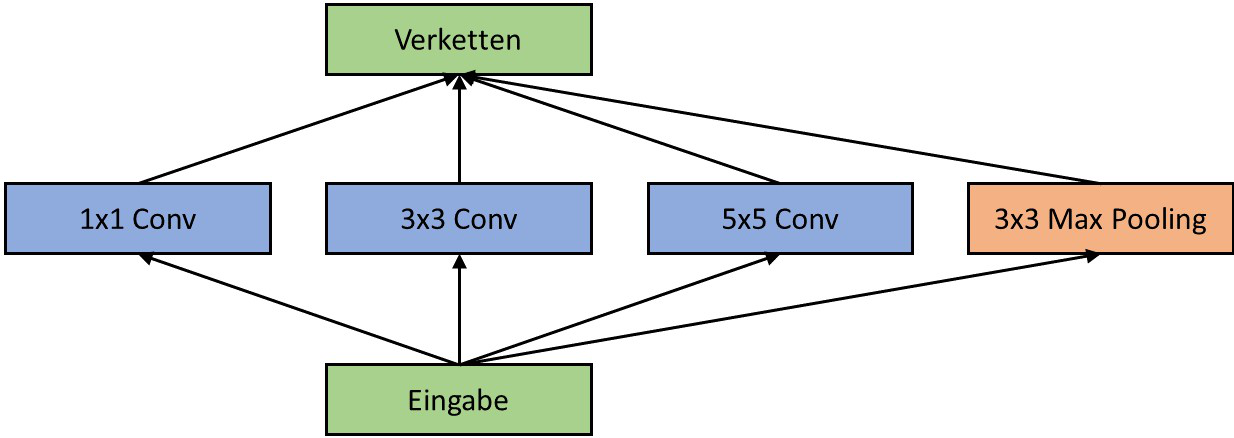
\includegraphics[width=12cm]{98_images/inception_layer1.png}
\caption{Aufbau des Inception Layer nach \cite{going-deeper-with-convolutions} ohne 1x1 Convolution.}
\label{fig:inception1}
\end{figure}

Aufgrund des Rechenaufwands von 5x5 Convolutional Layern, kann die Architektur aus Abbildung \ref{fig:inception1} mit 1x1 Convolutional Schichten zum Aufbau in Abbildung \ref{fig:inception2} erweitert werden. Somit sinkt die benötigte Rechenleistung und es wird eine kleinere Dimension der Ausgabe erzielt. \cite{going-deeper-with-convolutions}

\begin{figure}[h!]
\centering
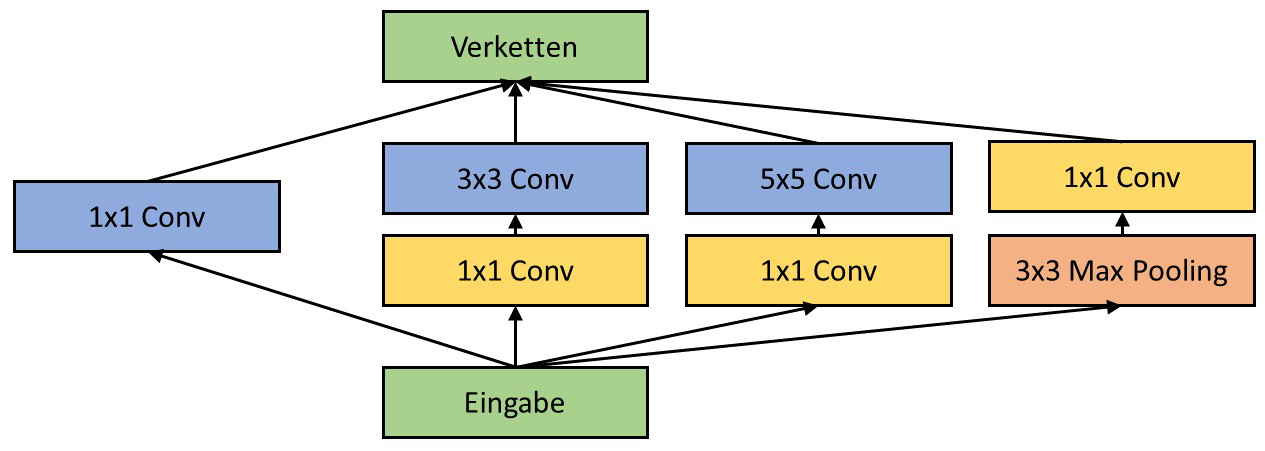
\includegraphics[width=12cm]{98_images/inception_layer2.png}
\caption{Aufbau des Inception Layer nach \cite{going-deeper-with-convolutions} mit 1x1 Convolution.}
\label{fig:inception2}
\end{figure}

\mypar Die Weiterentwicklung dieses Moduls hat zu einer Diversifikation bei den Varianten geführt. So entstanden die Inception-A, Inception-B, Inception-C, Reduction-A und Reduction-B Module. Im Vergleich zu den zwei Jahre älteren Versionen haben diese einen geringeren Trainingsaufwandaufwand. \cite{inception-inceptionresnet-and-the-impact-of-residual-connections-on-learning}


% Separable Convolution Layer
\subsubsection{Separable Convolution Layer}
Das Separable Convolution Layer ist, vom Aufbau her, ähnlich zu dem eines Inception Moduls, welches nur eine Größe von Filtern verwendet und keinen Pooling Layer besitzt. Dies kann als gesamte $1\times1$ Convolution, die von weiteren einzelnen Convolutional Layern gefolgt wird, gesehen werden. Die nachfolgenden Schichten arbeiten auf nichtüberlappenden Segmenten der Ausgabe. Beide Operationen werden von einer ReLU-Aktivierungsfunktion gefolgt. Ein Beispiel für eine solche Architektur ist in Abbildung \ref{fig:sep_conv} aufgezeigt. \cite{xception-dl-with-depthwise-sep-conv}

\begin{figure}[h!]
\centering
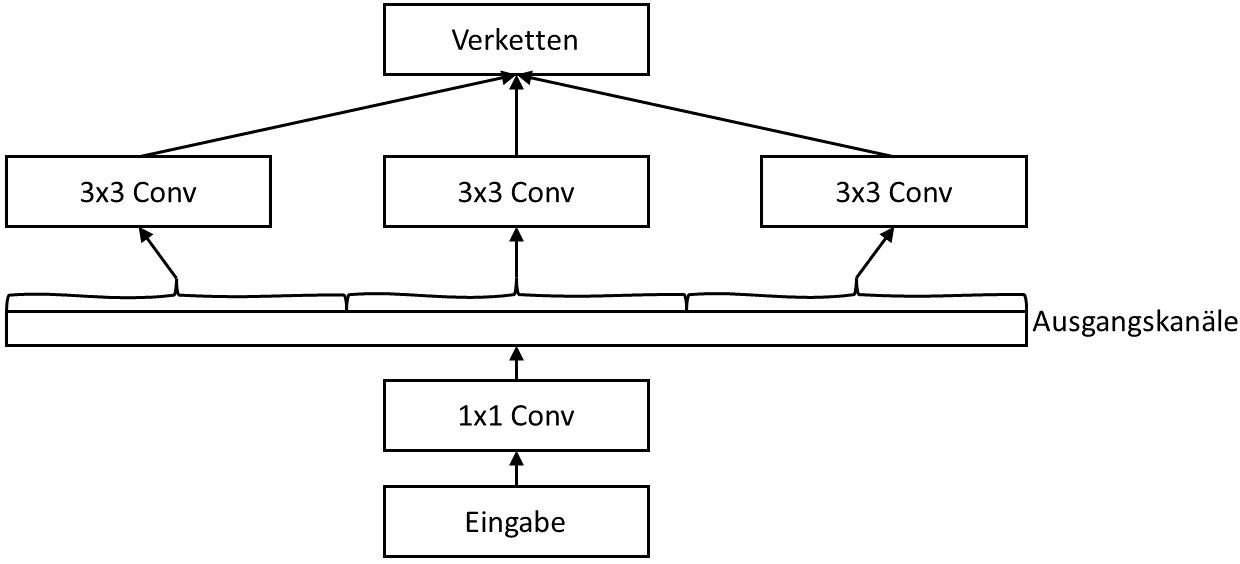
\includegraphics[width=12cm]{98_images/sep_conv.png}
\caption{Beispiel eines Separable Convolution Layer nach \cite{xception-dl-with-depthwise-sep-conv}}
\label{fig:sep_conv}
\end{figure}


% Residual Layer
\subsubsection{Residual Layer}
Beim sogenannten Residual Layer werden mehrere Convolutional und Batch Normalization Layer hintereinander gestellt und es wird eine sogenannte ''Identitätsverknüpfungsverbindung'', die auch als Abkürzung (engl. Shortcut) bezeichnet wird, eingeführt. Shortcut-Verbindungen überspringen eine oder mehrere Schichten. In diesem Fall wird diese Verbindung so verwendet, dass ihr Ausgang mit dem Ausgang der gestapelten Schichten addiert wird. Hierbei müssen beide Größen von der gleichen Dimension sein. Die Struktur ist in Abbildung \ref{fig:residual}(a) dargestellt. \cite{deep-residual-learning}

\begin{figure}[h!]
\centering
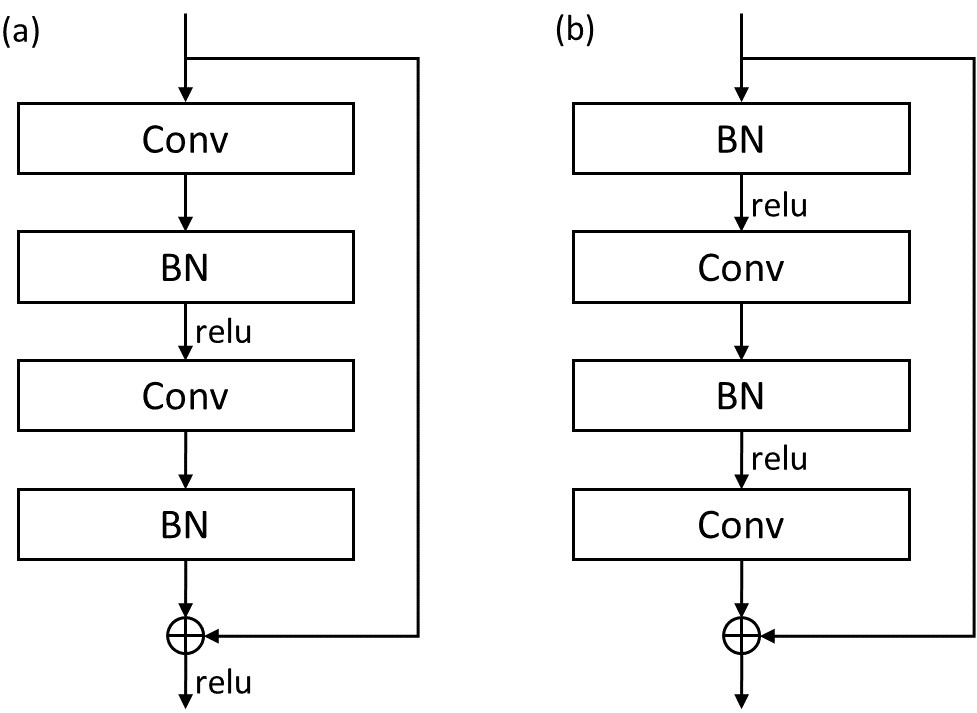
\includegraphics[width=8cm]{98_images/residual_layers.png}
\caption{(a) Aufbau des originellen Residual Layers nach \cite{deep-residual-learning}; (b) Aufbau der Weiterentwicklung eines Residual Layers \cite{identity-mappings-in-drn}.}
\label{fig:residual}
\end{figure}

\mypar Ein Jahr nach der Einführung des Residual Layers führte He et. al \cite{identity-mappings-in-drn} eine verbesserte Version ein. Ihr Aufbau ist in Abbildung \ref{fig:residual}(b) aufgezeigt. Hiermit wurde der Fehler auf den CIFAR-10-Datensatz, welches aus 60.000 Bilder aus 10 Klassen besteht \cite{krizhevsky2009learning}, von 7,61\% auf 4,92\% verringert. \cite{identity-mappings-in-drn}


% Bottleneck Layer
\subsubsection{Bottleneck Layer}
Das Bottleneck Layer (siehe Abbildung \ref{fig:bottleneck}) ist die nächste Entwicklung des ursprünglichen Residual Layers und besteht aus drei hintereinanderliegenden Convolutional Layer mit Filtern der Größen $1\times1$, $3\times3$ und $1\times1$. Die Schichten mit den $1\times1$ Filtern reduzieren erst und erhöhen dann die Dimensionen, somit hat die mittlere Schicht mit dem $3\times3$ Filter eine kleinere Ein- und Ausgangsdimension. Dieser Aufbau erinnert an einem Flaschenhals (engl. Bottleneck), woran der Name des Filters angelehnt ist. Die parameterfreie Verzweigung, die an den zwei Enden mit den höchsten Dimensionen verbunden ist, führt außerdem zu einem geringeren Zeitverbrauch. \cite{deep-residual-learning}

\begin{figure}[h!]
\centering
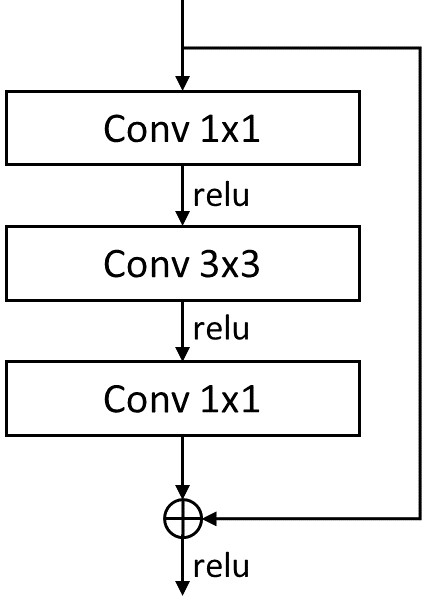
\includegraphics[width=3.5cm]{98_images/bottleneck_layer.png}
\caption{Aufbau eines Bottleneck Layers nach \cite{deep-residual-learning}.}
\label{fig:bottleneck}
\end{figure}


% Inverted Residual Layer
\subsubsection{Inverted Residual Layer}\label{inv-res-layer-section}
Ein Inverted Residual Layer, auch MBConv Layer genannt, besteht aus einer $1\times1$ Convolution, einer $3\times3$ Depthwise Convolution (kurz DepthConv), einer weiteren 1x1 Convolution und einer Shortcut-Verbindung vom Eingang des Layers bis zum Ausgang der zweiten $1\times1$ Convolution. In Abbildung \ref{fig:mbconv} ist dieser Aufbau zu sehen. Die Depthwise Convolution in der Mitte funktioniert ähnlich zu einer normalen Convolution. Der Unterschied liegt darin, dass der Filter auf den einzelnen Informationskanälen angewendet wird. Erst wird die Eingabe und der Filter in den Kanälen gespalten. Daraufhin wird der Filter angewendet und zuletzt werden die Ausgaben zusammengestellt. Diese Operation vermindert die Anzahl an Parametern. \cite{mobilenetv2}

\begin{figure}[h!]
\centering
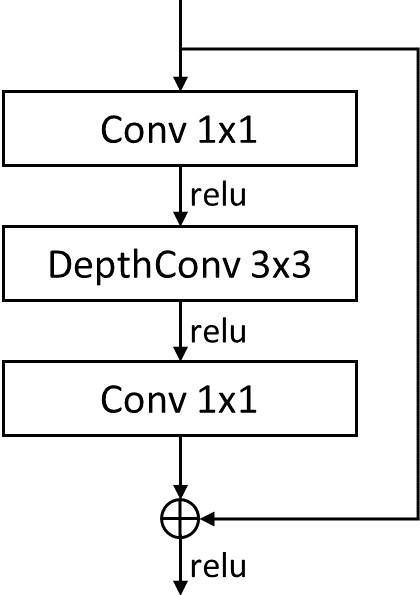
\includegraphics[width=3.5cm]{98_images/inverted_residual_layer.png}
\caption{Zusammenstellung des Inverted Residual Layer \cite{mobilenetv2}.}
\label{fig:mbconv}
\end{figure}



%
% 2.3.3 CNN Architekturen
%
\section{Netzwerkarchitekturen}\label{sec:architekturen-grundlagen}
Seit der Einführung von CNNs wurden viele unterschiedliche Architekturen für diverse Zwecke entworfen. Somit ist im Laufe der Zeit die Komplexität, aber auch die Leistung gestiegen. Dies ist am Beispiel von ImageNet ersichtlich. ImageNet ist ein Datensatz bestehend aus 14.197.122 annotierten Bildern aus unterschiedlichen Kategorien. In den letzten zehn Jahren ist die Genauigkeit des Modells mit dem besten Ergebnis von 50,9\% auf 90,2\% gestiegen (siehe Abbildung \ref{fig:imagenet}) \cite{imagenet-leaderboard}. Im Folgenden werden einige der in den letzten Jahren entworfenen Architekturen nach deren Veröffentlichungsjahr aufgezeigt.

\begin{figure}[h!]
\centering
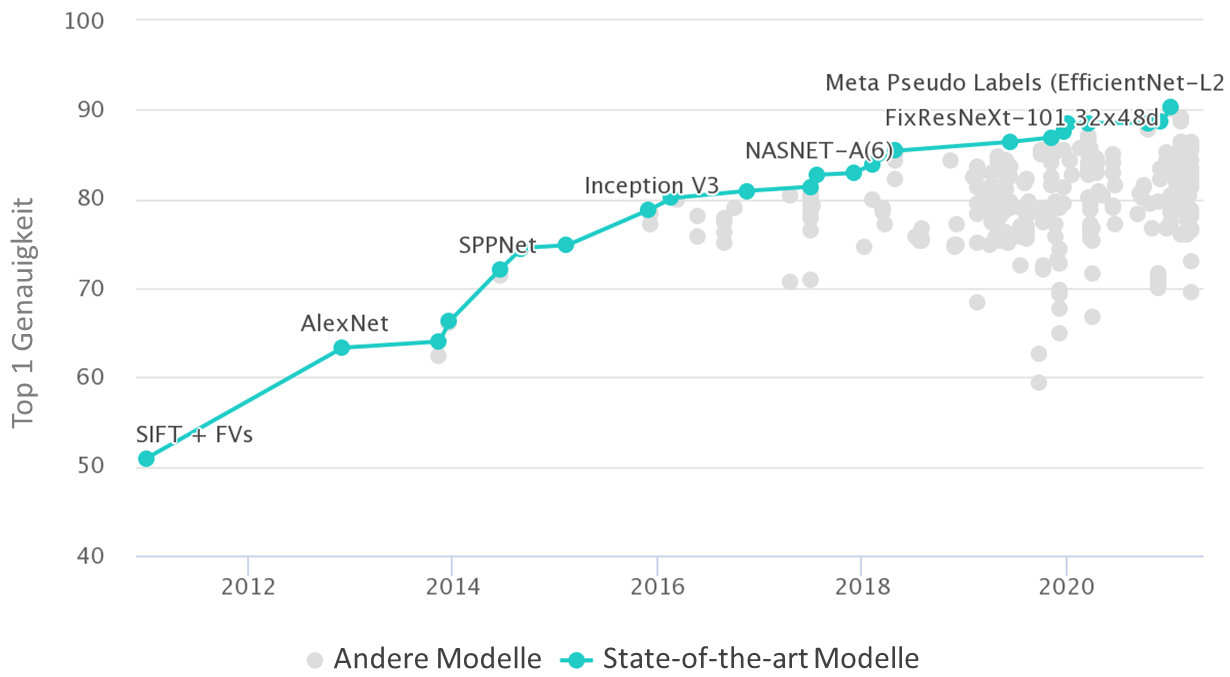
\includegraphics[width=14cm]{98_images/imagenet.png}
\caption{Rangliste für Modellergebnisse auf ImageNet über die Zeit \cite{imagenet-leaderboard}.}
\label{fig:imagenet}
\end{figure}


% AlexNet
\subsection{AlexNet}
Die von Krizhevsky et al. \cite{imagenet-class-w-deep-cnns} entworfene AlexNet-Architektur ist ein tieferes und breiteres Modell als das von LeCun \cite{lenet-2} veröffentlichte LeNet-5 CNN. AlexNet erreichte 2012 den State of the Art bei der Erkennungsgenauigkeit von Bildern und stellte einen Durchbruch in den Bereichen des Maschinellen Lernens und der Computer Vision dar \cite {the-history-began-from-alexnet}.


% VGG
\subsection{VGG}\label{sec:vgg-sec}
Das Visual Geometry Group (VGG) wurde von der Arbeitsgruppe, die diesen Namen an der University of Oxford trägt, entworfen. Es ist eine Weiterentwicklung des AlexNet und ist nach den gleichen Prinzipien aufgebaut, wie die Netze aus Ciresan et al. \cite{fleixble-hp-cnns-for-image-classification} und Krizhevsky et al. \cite{imagenet-class-w-deep-cnns}. Die zwei Varianten des Netzes, das VGG16 und das VGG19 unterscheiden sich in der Anzahl an enthaltenen Convolutional Layern, also in der Tiefe des faltenden neuronalen Netzes. Hierbei steht die Zahl am Ende der Namen für die Anzahl an Schichten mit Parametern, die Teil der Architekturen sind. \cite{very-deep-cnns-for-large-scale-img-recognition}

\mypar Ein großer Unterschied zu den neuronalen Netzen die bis 2013 den State of the Art repräsentierten, ist die Größe des Filters im ersten Convolutional Layer. Im Gegensatz zu den Filtern der Größe $11\times11$ mit einem Stride von vier in \cite{imagenet-class-w-deep-cnns}, wird im gesamten Netz eine $3\times3$ Größe mit Stride eins bevorzugt.

\mypar Laut Krizhevsky et al. \cite{very-deep-cnns-for-large-scale-img-recognition} besitzen zwei der $3\times3$ Convolutional Layer ein effektiveres Empfangsfeld als das eines $5\times5$ Layers; drei dieser Schichten besitzen das Empfangsfeld einer $7\times7$ Schicht, wie in \cite{visualizing-and-understanding-cnns}. Dies führt zu einer starken Reduzierung der Anzahl an Parametern. Für einen Stapel mit drei Convolutional Layern mit Filtern der Größe $3\times3$ mit $C$ Informationskanälen ergeben sich

\begin{equation}\label{eq:vgg1}
3(3^2C^2)=27C^2
\end{equation}

Parameter. Im Vergleich dazu, beträgt die Anzahl an Parametern bei nur einer Schicht mit $7\times7$ Filtern

\begin{equation}\label{eq:vgg2}
7^2C^2=49C^2.
\end{equation}


% ResNet
\subsection{ResNet}
Seit der Einführung der AlexNet-Architektur gehen neue neuronale Netze immer tiefer. So stieg die Anzahl an enthaltenen Convolutional Layern im Laufe der Jahre. 2012 hatte AlexNet \cite{imagenet-class-w-deep-cnns} fünf Convolutional Layer, drei Jahre später ist die Anzahl auf 16 mit dem VGG \cite{very-deep-cnns-for-large-scale-img-recognition} gestiegen.

\mypar Um eine Erhöhung der Tiefe des Netzes zu erzielen, ist es allerdings nicht ausreichend, weitere Schichten aufeinander zu stapeln. Bei tiefen Netzen tritt nämlich das sogenannte verschwindende Gradientenproblem \cite{drn-and-weight-initialization} auf, weshalb sie schwieriger zu trainieren sind. Der Gradient wird auf frühere Schichten zurück propagiert und kann, infolge wiederholten Multiplikationen, unendlich klein werden. Da das Netz tiefer und tiefer geht, wird dessen Leistung gesättigt oder nimmt schnell ab. Dies ist anhand des Beispiels aus Abbildung \ref{fig:error_deeper_networks} ersichtlich, bei dem das tiefere der beiden Netze eine schlechtere Leistung auf dem CIFAR-10-Datensatz erbrachte. 

\begin{figure}[h!]
\centering
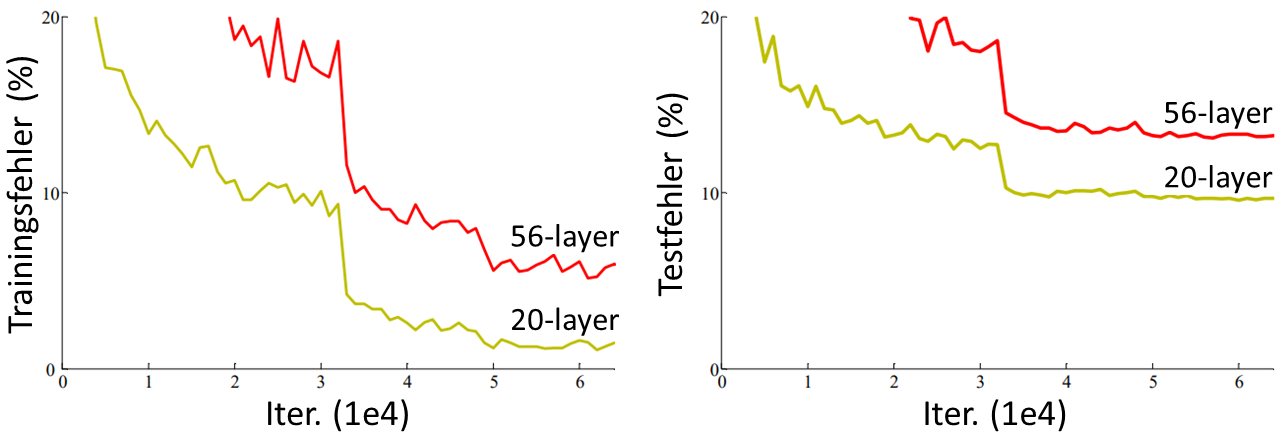
\includegraphics[width=12cm]{98_images/deeper_networks_example.png}
\caption{Trainingsfehler (links) und Testfehler (rechts) auf dem CIFAR-10-Datensatz mit ''einfachen'' Netzen mit 20 und 56 Schichten. Entnommen und Beschriftung übersetzt aus \cite{deep-residual-learning}.}
\label{fig:error_deeper_networks}
\end{figure}

\mypar Um dieses Problem zu beseitigen, werden Identitätsverknüpfungsverbindungen im Residual Layer eingeführt. Diese Schichten gelten als grundlegende Bausteine der Residual Networks, oder ResNets. Die Resnet50 und ResNet101 Architekturen nutzen das Bottleneck Layer, welches eine Weiterentwicklung des Residual Layers ist. \cite{deep-residual-learning}


% Inception-v4
\subsection{Inception-v4}
Inception-v4 \cite{inception-inceptionresnet-and-the-impact-of-residual-connections-on-learning} ist die vierte Generation der von Google entworfenen Inception-Architektur. Das Inception Layer wurde zum ersten Mal 2014 von Szegedy et al. \cite{going-deeper-with-convolutions} mit Inception-v1, oder GoogLeNet als Huldigung an Yann LeCuns LeNet-5 \cite{lenet-2}, eingeführt. In diesem Jahr gewann diese Architektur die Large Scale Visual Recognition Challenge (kurz: ILSVRC2014). Inception-v2 \cite{rethinking-inception-for-computer-vision} implentierte Batch Normalization und erzetzte die $5\times5$ Convolutional Layern durch zwei $3\times3$ Schichten, um die Anzahl an Parametern zu reduzieren. In der gleichen Veröffentlichung wurde ebenfalls die Inception-v3-Architektur \cite{rethinking-inception-for-computer-vision} eingeführt.

\mypar Die Prämisse für Inception-v4 ist das Erschaffen einheitlicherer Module. Zudem waren einige Module der früheren Entwicklung komplizierter als nötig. Hierfür wurde der ''Stem'', welcher die Operation vor den Inception-Blöcken darstellt, verändert. Zudem wurden die drei Hauptmodule Inception-A, -B und -C aktualisiert und es wurden sogenannte ''grid-reduction'' Module eingeführt, um die Breite und Höhe des Gitters zu verändern. \cite{inception-inceptionresnet-and-the-impact-of-residual-connections-on-learning}


% Inception-ResNet-v2
\subsection{Inception-ResNet-v2}
Inception-ResNet-v2 ist ein Convolutional Neural Network, welches auf der Inception-Architektur basiert und die Identitätsverknüpfungsverbindung der ResNets einbaut. Um dies umzusetzen, müssen Ein- und Ausgang nach der Convolution von der gleichen Dimension sein. Dafür werden Convolutional Layer mit Filtern der Größe $1\times1$ nach den ursprünglichen Convolutions eingesetzt. In den Inception-ResNet-A, -B und -C Modulen wird das Pooling Layer durch den Shortcut ersetzt. \cite{inception-inceptionresnet-and-the-impact-of-residual-connections-on-learning}


% Xception
\subsection{Xception}
Die 2017 veröffentliche-Xception Architektur ist von der Inception-Architektur \cite{rethinking-inception-for-computer-vision} inspiriert worden. Ein wichtiger Bestandteil von Xception ist die Einführung des Separable Convolution Layer. Der Aufbau von Xception besteht aus drei grundlegenden Teilen; dem Eingang, dem mittleren Durchfluss, welcher acht Mal wiederholt wird, und dem Ausgang. \cite{xception-dl-with-depthwise-sep-conv}


% MobileNetV3
\subsection{MobileNetV3}
MobileNetV3 ist eine Weiterentwicklung des MobileNet aus \cite{mobilenets} und wurde für die Benutzung mit CPUs von Mobiltelefonen entworfen. Das neuronale Netz besteht aus mehreren Inverted Residual Layern (siehe Abschnitt \ref{inv-res-layer-section})  und führt eine neue Aktivierungsfunktion, ''h-swish'', ein. \cite{searching-for-mobilenetv3}

\begin{equation}\label{eq:swish}
f(x)=x \cdot \sigma(\beta x), \text{         mit } \sigma(z)= \frac{1}{1+e^{-z}}
\end{equation}

\mypar Die ursprüngliche Swish-Funktion wurde 2017 von Ramachandran et al. \cite{searching-for-act-functions} eingeführt und ist in Gleichung \ref{eq:swish} beschrieben. Hierbei ist $\beta$ ein änderbarer Parameter. Laut \cite{searching-for-mobilenetv3} stellt h-swish eine Verbesserung der ursprünglichen Swish-Funktion dar, da die Rechenzeit verringert wird. Diese wird in Formel \ref{eq:h-swish} aufgezeigt.

\begin{equation}\label{eq:h-swish}
\text{h-swish}(x)=x\frac{\text{min}(\text{max}(x+3, 0), 6)}{6}
\end{equation}


% EfficientNet
\subsection{EfficientNet}
Die Grundidee hinter der Architektur von EfficientNets ist das sogenannte Compound Scaling. Anstatt Netze anhand der Tiefe (Anzahl der Schichten), Breite (Anzahl der Informationskanäle) oder Bildgröße zu skalieren, werden alle drei Dimensionen so verändert, dass sie ein Gleichgewicht bilden. Somit kann eine bessere Genauigkeit und Effizienz bei den neuronalen Netzen erzielt werden. Diese Methode kann auch bei anderen Architekturen angewendet werden. So wurde gezeigt, dass das Compound Scaling bei MobileNetV1, MobileNetV2 und ResNet-50 zu besseren Ergebnissen auf dem Imagenet-Datensatz führte. \cite{efficientnet}

\begin{equation}\label{eq:compound-scaling}
\begin{aligned}
\text{Tiefe: } d = \alpha^{\phi} \\
\text{Breite: } w = \beta^{\phi} \\
\text{Auflösung: } r = \gamma^{\phi} \\
\text{$\forall$ } \alpha \cdot \beta^2 \cdot \gamma^2 \approx 2, \alpha \geqslant 1, \beta \geqslant 1, \gamma \geqslant 1
\end{aligned}
\end{equation}

\mypar Compound Scaling verwendet einen Koeffizienten $\phi$, um die Breite, Tiefe und Auflösung gemeinsam zu bestimmen. Die Gleichungen aus \ref{eq:compound-scaling} beschreiben die skalierten Attribute. Der benutzerdefinierte Parameter $\phi$ bestimmt die zusätzlichen verfügbaren Ressourcen und $\alpha$, $\beta$ und $\gamma$ bestimmen die Verteilung dieser Ressourcen über der Tiefe $d$, Breite $w$ und Auflösung $r$. 

\begin{figure}[h!]
\centering
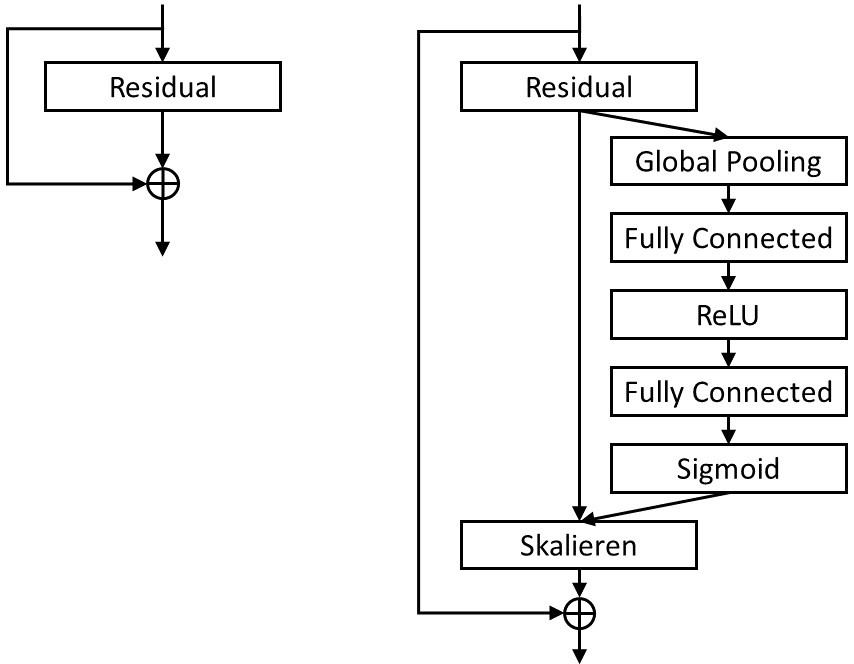
\includegraphics[width=10cm]{98_images/se_block.png}
\caption{Aufbau eines Residual Layers (links) und dem SE-ResNet Modul (rechts) nach \cite{squeeze-and-excitation-networks}.}
\label{fig:se-block-architecture}
\end{figure}

\mypar Der Hauptbaustein des EfficientNet ist das Inverted Residual Layer, welches zusätzlich noch durch Squeeze-and-Excitation (SE) optimiert wird \cite{efficientnet}. Der SE-Block besitzt am Eingang eine Convolution. Mithilfe des Poolings wird jeder Informationskanal auf einen einzigen Wert zusammengepresst. Das darauffolgende Fully Connected Layer mit einer ReLU als Aktivierungsfunktion fügt eine Nichtlinearität ein und das zweite Fully Connected Layer glättet die Funktion. Dieses Layer verwendet die Sigmoid-Funktion. Am Ende wird jede Feature Map der Faltungsoperation anhand des Ergebnisses der hinzugefügten Schichten skaliert. Abbildung \ref{fig:se-block-architecture} zeigt die Umsetzung für ein Residual Layer. Diese zusätzliche Struktur benötigt unter 1{\%} an zusätzlicher Rechenleistung und kann zu jedem neuronalen Netzwerk hinzugefügt werden. \cite{squeeze-and-excitation-networks}














